\documentclass[10pt]{beamer}

\usepackage[utf8]{inputenc}
\usepackage{amsmath,amssymb,amsfonts,amsthm,mathrsfs}
\usepackage{mathtools}
\usepackage{hyperref}

\usepackage{verbatim}
\usepackage{graphicx}
\usepackage{scalefnt}
\usepackage{algorithmic}
\usepackage{tikz}
\usepackage{caption}
\usepackage{subcaption}
\newcommand{\inner}[2]{\langle{#1},{#2}\rangle}
\usepackage{multicol}
\setlength{\columnseprule}{0.4pt}
\DeclareMathOperator*{\aff}{aff}
\DeclareMathOperator*{\conv}{conv}
\DeclareMathOperator*{\cone}{cone}
\theoremstyle{definition}
\usepackage{bbm}
\usepackage{lmodern} %for institute name
\usepackage{hyperref}
\setcounter{MaxMatrixCols}{20}
\newtheorem{thm}{Theorem}
\newtheorem{prop}{Proposition}
\newtheorem{rem}{Remark}
\newtheorem{defn}{Definition}
\newtheorem{lem}{Lemma}

\everymath{\displaystyle}
\title{Tikhonov Regularization and Adversarial Robustness}
\author{Charlie}

% \institute{KTH Royal Institute of Technology}
\date{\today}

\usetheme{Copenhagen}
\usecolortheme{rose}

\let\olditem\item
\renewcommand{\item}{\setlength{\itemsep}{\fill}\olditem}

\begin{document}
\frame{\titlepage}

\begin{frame}{Localization}
\textbf{Common Sensors}
\begin{itemize}
    \item GPS: Uses time-of-flight to several satellites to estimate x/y/z position
    \item Gyroscope: Electromechanical device for determining the direction of gravity
    \item Accelerometer: Measures the angular acceleration
    \item Magnetometer: Uses a magnet to determine magnetic North
    \item IMU: Integrates gyroscope, accelerometer, magnetometer to determine location. 
\end{itemize}
The actual IMU and GPS algorithms are outside the scope of this presentation.
\end{frame}

\begin{frame}{Kalman Filter}
    Many techniques exist for filtering the data. The provided MATLAB code uses the standard kalman filter.
    
    $\bar{u}_k = u_k - \delta u_k + w_k$
    
    where $u_k$ is a signal, $w_k$ is an additive noise matrix, and $\delta u_k$ is a slowly varying measurement bias:
    
    $ \delta u_k = \delta u_{k-1} + w_k^*$

    and $w_k^*$ is an additive noise matrix with a specific covariance matrix, derived from the data. Each datapoint is then determined by another iterative function:
    $ u_{k+1} = f(u_k)$
    $$ u_k = u_{k-1} - \delta(\delta u_{k-2} + w_k^*) + w_k $$
    Our gyroscope has a known error of .01 degrees latitude per second, skewing North due to the angular momentum of the earth. In meters near the equator, .01 degree of latitude is approximately equal to 111 meters \footnote{\href{https://www.usna.edu/Users/oceano/pguth/md_help/html/approx_equivalents.htm}{USNA}}.  
\end{frame}

% TASK 1 Use the functions errorgrowth.m and Nav eq.m to evaluate how
% the position error grows with time. Assume that the navigation system is sta-
% tionary; the initial position and velocity is zero; the initial roll, pitch, and yaw
% are zero; the accelerometer measurements are error free; and the gyroscope
% measurements are error free except from a bias in the x-axis gyroscope with
% a magnitude of 0.01 ◦/s. Explain the observed behavior: In what directions
% do you get a position error? Find an approximative formula for the error
% behavior. Where is error largest, Stockholm or Lund?

\begin{frame}{Task 1: Error Growth}
\begin{figure}
    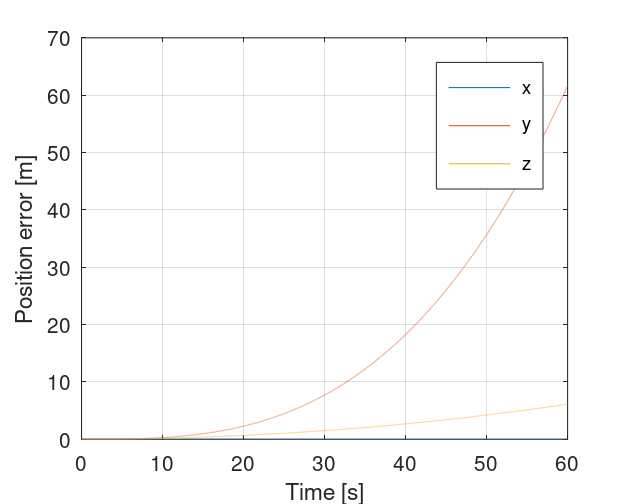
\includegraphics[width=.8\textwidth]{images/error_growth.png}
    \caption{Error Growth over time for unaided IMU.}
    \label{fig:my_label}
    We can see that, as expected, the error rate grows over time without bound.
\end{figure}
\end{frame}

\begin{frame}{Error Bias}
    This error arises from the uncertainty of the accelerometer since the accelerataion, $a$ in the $x,z$ directions is initialized as:
    $$
    a_x = 0, a_z = -g
    $$
    $$
    \delta a = 
    \begin{bmatrix}
        \delta a_x \\
        \delta a_z \\
    \end{bmatrix} = 
    \begin{bmatrix} 
        -g \delta a \\
        0           \\
    \end{bmatrix}
    \
    $$
    Integrating over the iterative function from the previous, we know that
    $$
    \delta a(t) = \delta u_0 + \int_0^t err_0 \cdot dt
    $$
    where the $err_0$ is the bias due to the gyroscope's assumption that gravity is truly straight down relative to the angular momentum of the planet. Because it isn't and because the earth spins east, our gyroscope is biased North as per the right hand rule meaning that we would expect a larger error in Ume\aa~than Stockholm or Lund.
\end{frame}
% TASK 2 Familiarize yourself with the Matlab code that implements the
% GNSS-aided INS and execute the script main.m. Modify the code to simulate
% a GNSS-receiver outage from 200 seconds and onward. Plot the estimated car
% position ˆxk (output data.x h). Also plot the difference between estimated
% car position and the GPS position without outage. Experiment with varying
% settings of filter parameters in get settings.m and try to improve the filter
% performance during GPS outage.
\begin{frame}{Task2}


\end{frame}

%  TASK 3 Implement support for non-holonomic motion constraints
% and speedometer measurements into the GNSS-aided INS framework.
% Some hints where changes are needed are given in the code. Turn
% off speedometer measurements and run with only the motion constraints
% (settings.speed aiding=’off’;settings.non holonomic=’on’ ). Tune
% the filter by changing the magnitude of filter parameters, for example R(3),
% until you get a decent performance and plot the position estimates and po-
% sition error, with GNSS outage. You should see a substantial improvement.

\begin{frame}{Task3}
    
\end{frame}
% TASK 4 The data included in the GNSSaidedINS.zip folder also include
% measurements from a speedometer. Let the fusion filter also use these mea-
% surements, trim the filter, and then plot the position estimates and position
% error, with GNSS outage. What is the resulting rms error of the position
% trajectory?
\begin{frame}{Task4}
    
\end{frame}

% \begin{frame}
% \frametitle{References}

% \setbeamertemplate{bibliography item}[text]

% \bibliographystyle{acm}
% \bibliography{mobility.bib}
% \end{frame}
\end{document}
